%% ── Section 3: Methodology ──────────────────────────────────
\section{Methodology}
\label{sec:method}

\subsection{Problem Formulation}

Let $K = 5$ participating hospital clients hold private datasets
$\mathcal{D}_k = \{(x_i, y_i)\}_{i=1}^{n_k}$ with retinal fundus images $x_i$
and ordinal grades $y_i \in \{0, 1, 2, 3, 4\}$. The objective is to collaboratively
train a shared EfficientNet-B3 global model parameterised by $w$ over $T$
communication rounds without ever transmitting $\mathcal{D}_k$ to a central server.
Heterogeneity causes the local empirical distributions $P_k(y)$ to diverge sharply
from the global distribution $P(y)$, resulting in severe client drift and weight
divergence during the local updating phase.

\subsection{Limitations of Nominal Objectives}

Standard FL approaches employ Cross-Entropy (CE) loss during local training.
Let $\mathbf{p}(x) \in \mathbb{R}^5$ be the softmax probabilities. The CE loss for
a true grade $y$ is $-\log p_y(x)$. Crucially, this formulation does not differentiate
between a model predicting $y+1$ or $y+4$; both are treated identically as incorrect
classes. In heavily skewed federated clients (e.g., a clinic with only Grade~0 patients),
CE loss rapidly forces the local decision boundaries to classify all incoming features
as Grade~0, destroying the network's previously learned ability to recognise severe
pathology.

\subsection{Distance-Aware OrdinalLoss}

To regularise local client models against ordinal degradation, we formulate a hybrid
objective, OrdinalLoss, applied during local client training:
\begin{equation}
\mathcal{L}_{\text{ord}}(f(x), y) =
  (1 - \lambda)\,\mathcal{L}_{\text{CE}}(f(x), y)
  + \lambda\,(\hat{y} - y)^2
\label{eq:ordloss}
\end{equation}
where $\mathcal{L}_{\text{CE}}$ is class-weighted cross-entropy with fixed empirical
weights $\mathbf{c} = [1.0, 5.0, 1.5, 10.0, 4.0]$ to counter natural dataset imbalance,
and $\lambda = 0.5$ balances the two terms. The parameter $\hat{y}$ is the
continuous expected grade under the softmax output distribution:
\begin{equation}
\hat{y} = \sum_{c=0}^{4} c \cdot p_c(x)
\label{eq:expgrade}
\end{equation}
The penalty term $(\hat{y} - y)^2$ scales quadratically with misclassification
distance. Misclassifying a Grade~4 proliferative case as Grade~0 incurs $16\times$
the penalty of predicting Grade~3. This strong continuous gradient forces local
optimisers to maintain globally aligned ordinal boundaries, even when the client's
local data is overwhelmingly skewed toward a single class.

\subsection{Server Validation Set $\mathcal{V}$ and QWK Estimation}

To dynamically assess client model quality without accessing private records, the
server maintains a compact validation set $\mathcal{V}$ comprising exactly 50 images
(10 images per grade, sampled uniformly from the independent DDR test split with
seed~42). Because $\mathcal{V}$ is strictly balanced across all five severity grades,
evaluation on this set provides an unbiased global measurement of ordinal discrimination
capability. At communication round $t$, after receiving locally updated weights
$\tilde{w}_k^t$, the server evaluates:
\begin{equation}
\kappa_k^t =
\mathrm{QWK}\!\left(\{y_i\}_{x_i \in \mathcal{V}},\,
\{\hat{y}_k^t(x_i)\}_{x_i \in \mathcal{V}}\right)
\label{eq:serverqwk}
\end{equation}

\subsection{Adaptive Cosine Schedule $\beta(t)$}

In early rounds, local updates produce high-variance predictions on $\mathcal{V}$
because the global representation space has not yet converged. Relying entirely on
QWK scores in round 1 would lead to erratic aggregation. We therefore dynamically
transition from stable sample-count weighting to quality-driven weighting using a
half-cosine annealing schedule:
\begin{equation}
\beta(t) = \beta_0 \cos\!\left(\frac{\pi (t - 1)}{2 (T - 1)}\right)
\label{eq:beta}
\end{equation}
where $\beta_0 = 0.9$ and $T = 10$. At $t=1$, $\beta(1) = 0.9$, heavily leveraging
traditional FedAvg sample-count stability. As training progresses to $t=T$,
$\beta(T) = 0$, transitioning entirely to quality-driven aggregation to filter out
diverged clients.

\subsection{QWK-Weighted Aggregation}

The scalar aggregation weight $\omega_k^t$ for client $k$ at round $t$ is:
\begin{equation}
\omega_k^t =
\beta(t)\,\frac{n_k}{\sum_j n_j}
+ (1 - \beta(t))\,\frac{\max(0, \kappa_k^t)}{\sum_j \max(0, \kappa_j^t)}
\label{eq:hybrid}
\end{equation}
Negative $\kappa_k^t$ values are clamped to zero, excluding catastrophically
collapsed client models from aggregation entirely. The server then computes the
global update as $w^{t+1} = \sum_{k=1}^{K} \omega_k^t \tilde{w}_k^t$. The
complete procedure is detailed in Algorithm~\ref{alg:ordinalfed}.

\begin{algorithm}[t]
\caption{OrdinalFed Training Pipeline}
\label{alg:ordinalfed}
\small
\begin{algorithmic}[1]
\REQUIRE Clients $K$, rounds $T$, local epochs $E$, trade-off $\lambda$,
         initial schedule $\beta_0$, server set $\mathcal{V}$, initial weights $w^0$.
\FOR{$t = 1$ \TO $T$}
  \STATE Broadcast global model $w^t$ to all clients $k \in \{1,\ldots,K\}$
  \FOR{each client $k \in \{1,\ldots,K\}$ \textbf{in parallel}}
    \STATE $\tilde{w}_k^t \leftarrow \textsc{LocalTrain}(w^t, \mathcal{D}_k, E, \lambda)$
           \hfill\textit{(Eq.~\ref{eq:ordloss})}
    \STATE Evaluate validation score $\kappa_k^t$ on $\mathcal{V}$
           \hfill\textit{(Eq.~\ref{eq:serverqwk})}
  \ENDFOR
  \STATE Compute annealing factor $\beta(t)$
         \hfill\textit{(Eq.~\ref{eq:beta})}
  \STATE Compute aggregation weights $\omega_k^t$ for all $k$
         \hfill\textit{(Eq.~\ref{eq:hybrid})}
  \STATE $w^{t+1} \leftarrow \sum_{k=1}^{K} \omega_k^t \tilde{w}_k^t$
\ENDFOR
\RETURN Final model $w^T$
\end{algorithmic}
\end{algorithm}

%% FULL-WIDTH FIGURE: QWK Trajectories
\begin{figure*}[t]
  \centering
  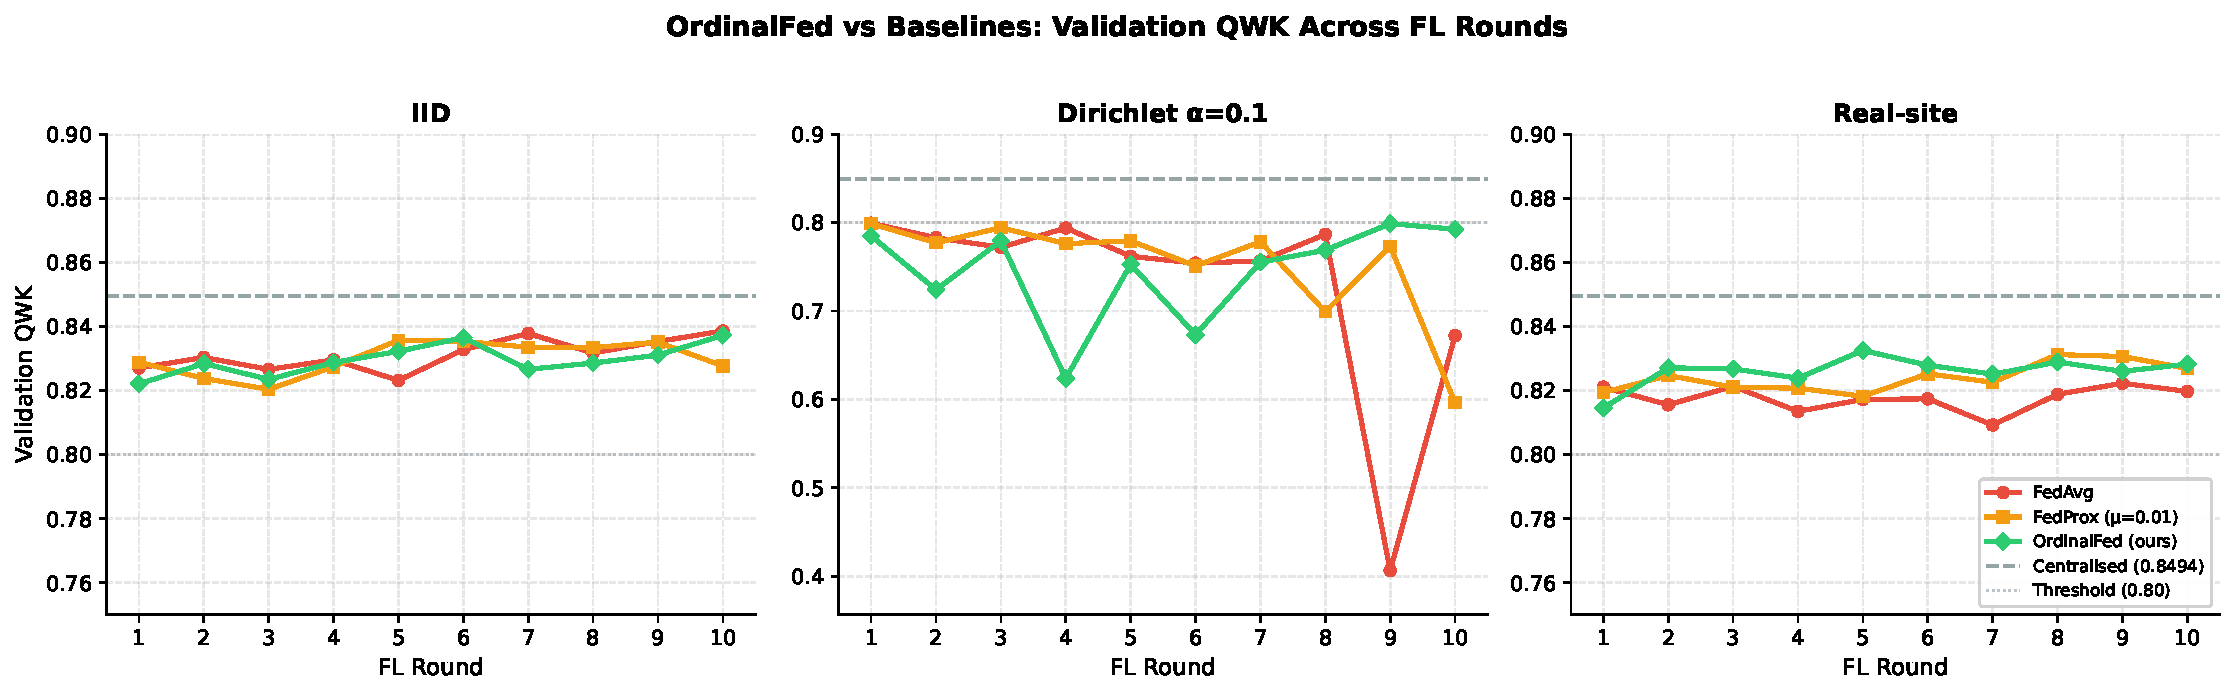
\includegraphics[width=\textwidth]{fig4_qwk_combined.pdf}
  \caption{\normalsize Validation QWK trajectories across 10 communication rounds for
  IID, Dirichlet ($\alpha=0.1$), and real-site partitions. While FedAvg
  and FedProx suffer catastrophic collapse under extreme skew ($\alpha=0.1$),
  OrdinalFed (green curve) maintains robust stability ($\mathrm{QWK} \geq 0.6238$)
  while achieving the highest peak performance in the realistic real-site partition.}
  \label{fig:qwk_curves}
\end{figure*}
